\clearpage
\thispagestyle{empty}
\null
\newpage
\cleardoublepage
\phantomsection
\markboth{\spacedlowsmallcaps{Appendices}}{\spacedlowsmallcaps{Appendices}}
\part*{Appendices}
\label{part:annexes}
\clearpage
\thispagestyle {empty}
\null
\newpage
\chapter{Notations of the MAMAD method}\label{appendix:notations}
\section{General notations}
\begin{itemize}
       \item $S$: set of possible states.
       \item $A_i$, $A$: set of actions of agent $i$, and joint set of actions.

       \item $\Omega_i$, $\Omega$: space of observations of agent $i$, and joint space.
       \item $H$, $H^{joint}$: set of individual and joint histories.
       \item $T$, $T_j$: transition function of the environment or digital twin.

       \item $R$, $R^E_t$, $R^G_t$, $R^j_H$: reward function (general, per environment, per objective, or based on histories).
       \item $\gamma \in [0,1]$: discount factor.

       \item $\pi_i$, $\pi$, $\pi^{joint}$: individual policy, global policy, joint policy.
       \item $\pi^*$: optimal policy.

       \item $V^\pi$, $V^{\pi^j}_{T_j}$: value function or adapted observation-value function.
       \item $d \in D$: a Dec-POMDP defined as $d = (S,\{A_i\},T,R,\{\Omega_i\},O,\gamma)$.
       \item $d \in OD$: an Observation-based Dec-POMDP (ODec-POMDP) defined as $d = (\Omega, A, \mathcal{T}^j, \Omega^{\mathcal{T}^j}_0, R^j_H, S^j_H, \texttt{Render}^j_H, \gamma)$.

       \item $\tilde{h}_t$: recurrent hidden state estimated by the World Model.
\end{itemize}
\section{Notations for the modeling activity (MOD)}
\begin{itemize}
       \item $G_{\text{inf}}$: informal global objective.
       \item $S_{\text{inf}}$: informal organizational constraints.

       \item $E$: description of the real environment.
       \item $\Omega^j_0$: set of joint initial observations.
       \item $(Enc, Dec)$: autoencoder used to compress and reconstruct observations.
       \item $z_t$: latent representation of an observation.
       \item $T_z$: recurrent latent dynamic model (RLDM).
       \item $T_j(h,\omega,a) = \langle \tilde{h}‘, P(\omega’|h,\omega,a)\rangle$: JOPM predicting the next observation and updating the hidden state.
       \item $S^j_H$: stop function based on histories.

       \item $Render^j_H$: optional trajectory rendering function.
       \item $DH_j$: set of joint histories used for training.
\end{itemize}
\section{Notations for training activity (TRN)}
\begin{itemize}
       \item $MM = \langle OS, ar, rcg, gcg, rag, rrg, grg \rangle$: MOISE+MARL specification.
       \item $ar: A \to R$: relation assigning agents to roles.
       \item $rcg: R \to \{rag, rrg\}$: relation associating a role with a constraint guide.

       \item $gcg: G \to grg$: relation linking an objective to a constraint.
       \item $rag(h,\omega)$: expected action guide.
       \item $rrg(h,\omega,a)$: role reward guide.
       \item $grg(h)$: objective reward guide.

       \item $\rho_i$: role assigned to agent $i$.
       \item $m \in M$, $G_m$: mission $m$ and its associated objectives.
       \item $cht$: probability of strict compliance with a role.
       \item $B$: experience buffer (encoded transitions).
\end{itemize}
\section{Ratings for the analysis activity (ANL)}
\begin{itemize}
       \item $OF$: Organizational Fit (overall organizational fit).
       \item $SOF$, $FOF$: Structural and Functional Organizational Fit.

       \item $D_{trans}$: set of transition sequences $(\omega_t, a_t, \omega_{t+1})$.
       \item $D_{obs}$: set of observation sequences $(\omega_t)$.
       \item $p \in P$: Trajectory-based Pattern.

       \item $sl = \langle h, \{c_{min},c_{max}\}\rangle$: leaf sequence (history-cardinality).
       \item $sn = \langle \langle sl_1, sl_2, ...\rangle, \{c_{min},c_{max}\}\rangle$: node sequence.

       \item $l \in L$: label assigned to an observation or action.
       \item $bg: H \to \{0,1\}$: function testing whether a history belongs to a set $H_g$.
\end{itemize}
\section{Notations for transfer activity (TRF)}
\begin{itemize}
       \item $\pi^{\text {latest}}_j$: most recent joint policy.
       \item $need\_update$: signal indicating the need for an update.
       \item $launch\_update()$: procedure triggering the update of the model/policy.

       \item $batch\_size$: minimum size of $B$ to trigger an update.
       \item Deployment modes: DIRECT (local), REMOTE (distant).
\end{itemize}
\clearpage
\thispagestyle{empty}
\null
\newpage
\chapter{Additional details about CybMASDE}
\section{CybMASDE graphical interface}\label{appendix:cybmasde-gui}
\acn{CybMASDE} offers a web-based graphical interface developed with the Angular framework, allowing users to configure, execute, and analyze projects interactively. This interface offers an alternative to command line interface (CLI) use, while retaining the ability to automate processes via scripts. Figures \autoref{fig:cybmasde_screenshot_configuration}, \autoref{fig:cybmasde_screenshot_training}, \autoref{fig:cybmasde_screenshot_analyzing}, and \autoref{fig:cybmasde_refining_screenshot} illustrate the tabs dedicated to project configuration, policy training, analysis of trained policies, and policy refinement and transfer, respectively.
\begin{figure}[h!]
       \centering

       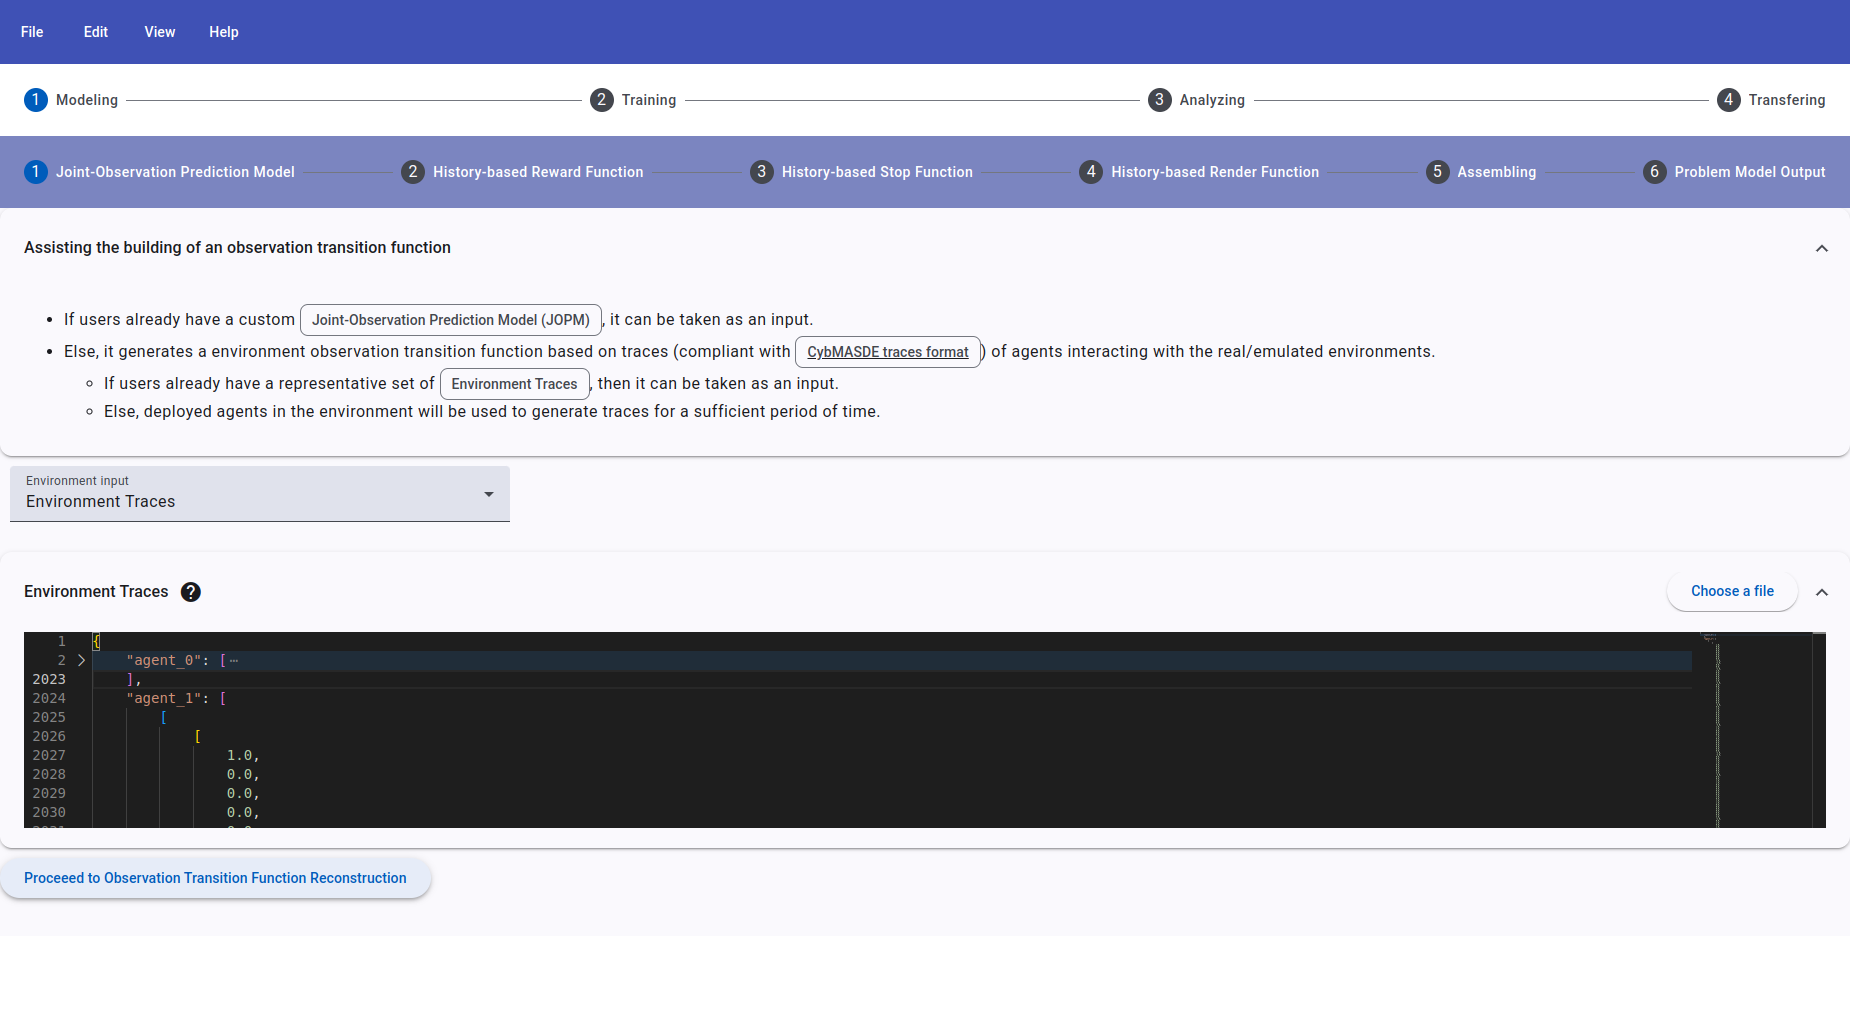
\includegraphics[width=\linewidth]{figures/CybMASDE_2.png}
       \caption[Screenshot of the modeling tab of the CybMASDE GUI]{Screenshot of the CybMASDE project configuration file editing GUI, showing the tab dedicated to modeling. In this tab, the user can configure parameters related to environment modeling, such as the choice between a handcrafted environment or one based on a World Model, as well as the hyperparameters associated with the deep learning models used for modeling.}

       \label{fig:cybmasde_screenshot_configuration}
\end{figure}
\begin{figure}[h!]
       \centering

       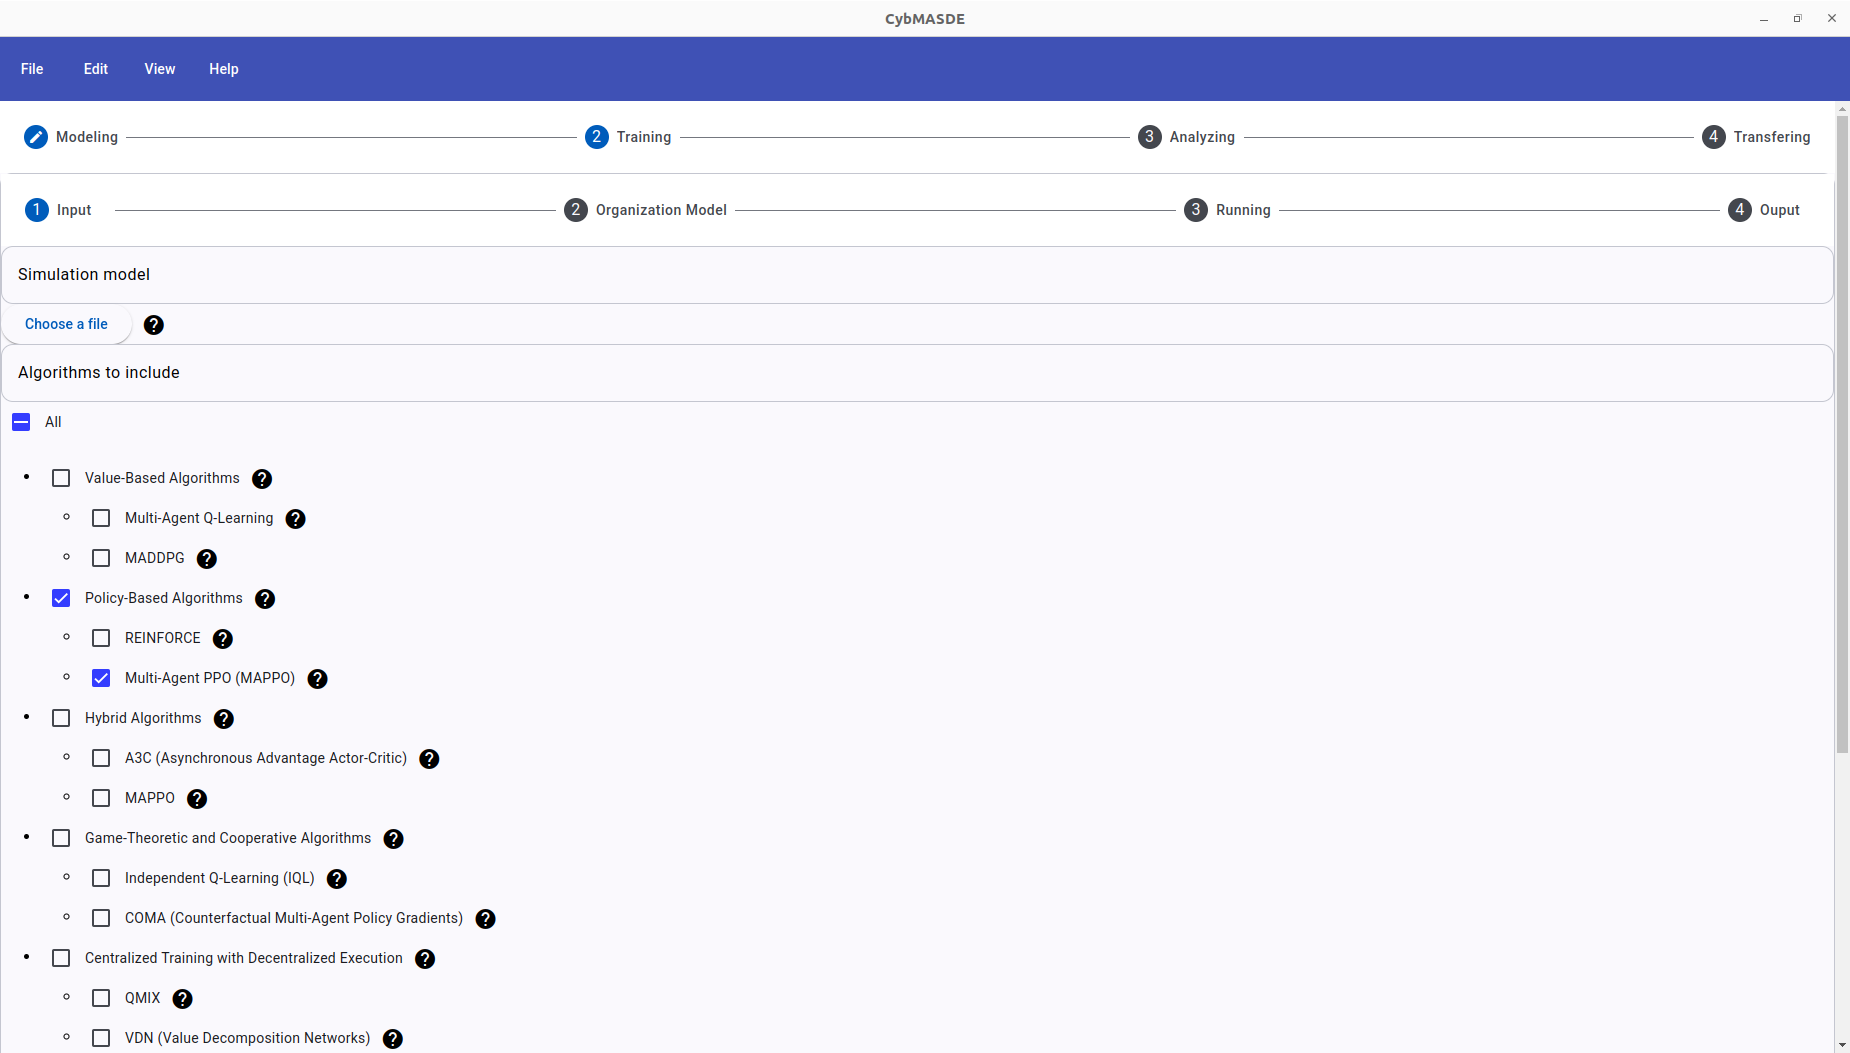
\includegraphics[width=\linewidth]{figures/training_screenshot.png}
       \caption[Screenshot of the training tab of the CybMASDE GUI]{Screenshot of the CybMASDE project configuration file editing GUI, showing the training tab. In this tab, users can configure parameters related to multi-agent policy training, such as the choice of MARL algorithm, training hyperparameters (batch size, learning rate, discount factor, etc.), and MOISE+MARL organizational specifications.}
       \label{fig:cybmasde_screenshot_training}
\end{figure}
\begin{figure}[h!]
       \centering
       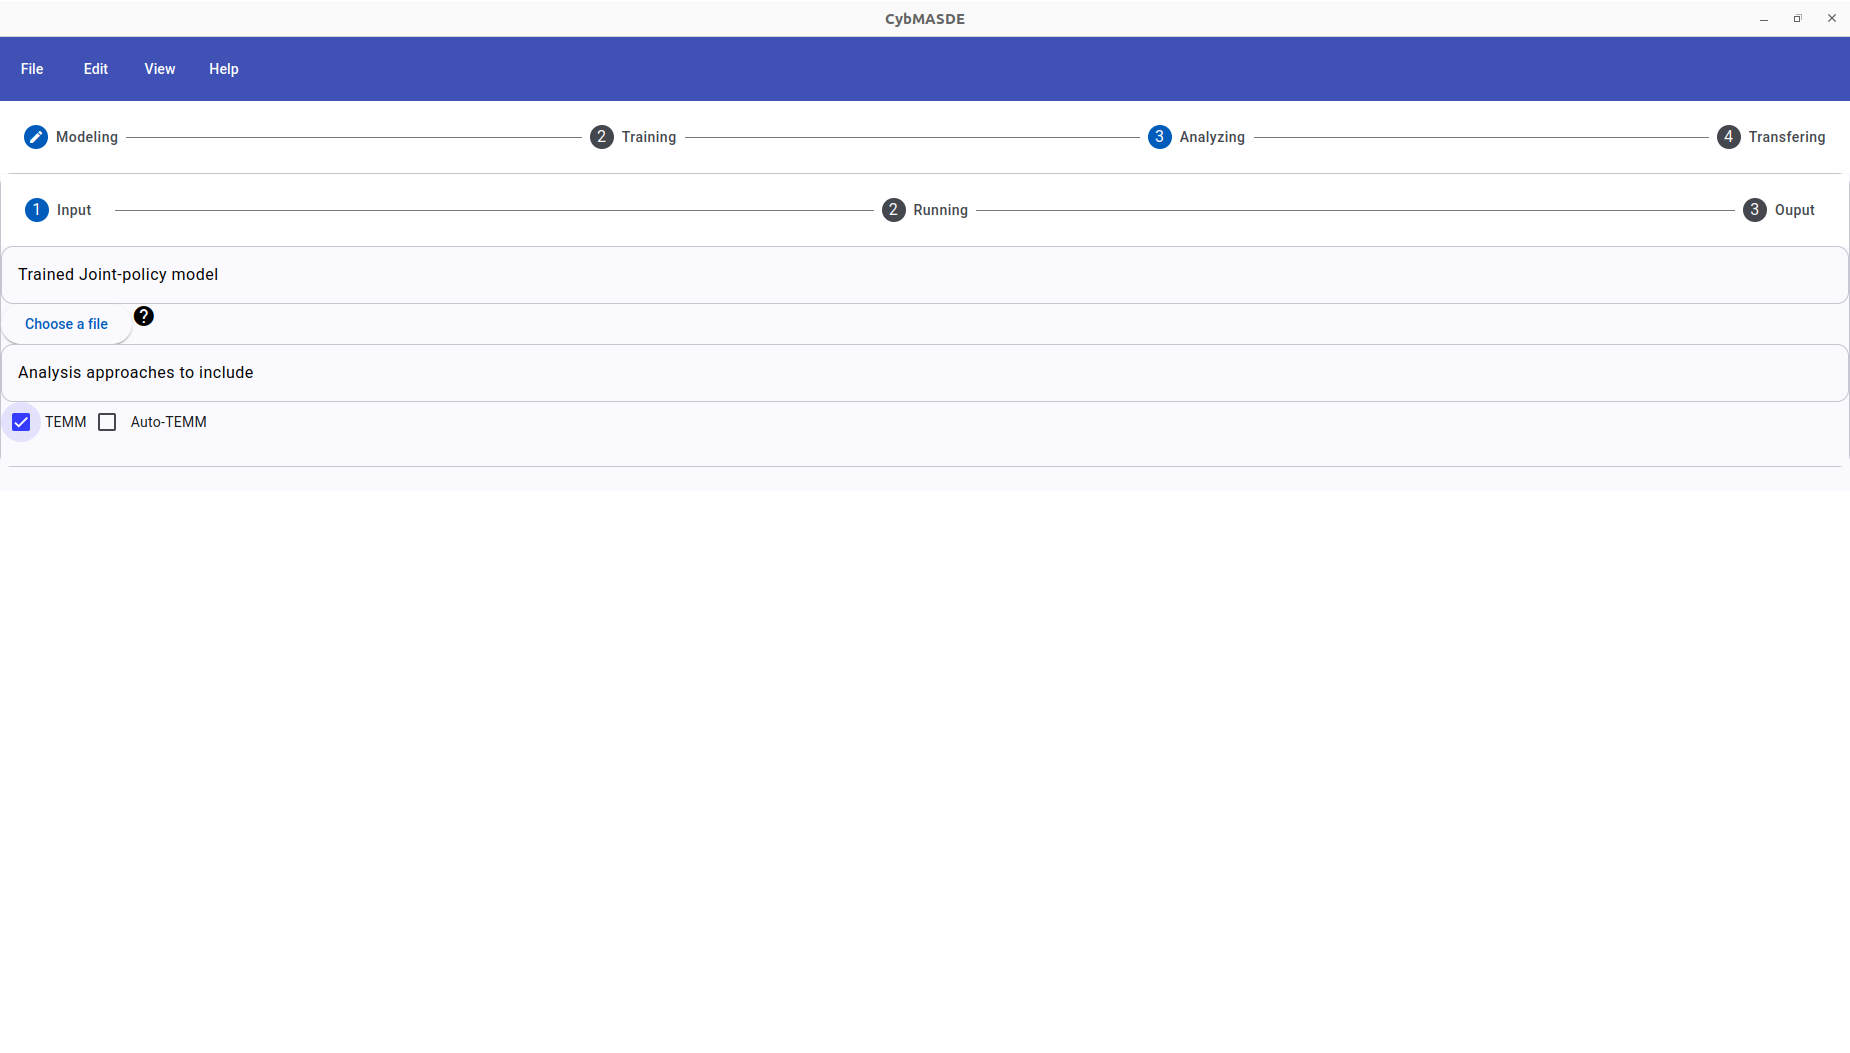
\includegraphics[width=\linewidth]{figures/analyzing_screenshot.png}
       \caption[Screenshot of the analysis tab of the CybMASDE GUI]{Screenshot of the CybMASDE project configuration file editing GUI, showing the analysis tab. In this tab, the user can configure parameters related to the analysis of multi-agent policies, such as the method to be used (\acn{TEMM} or \acn{Auto-TEMM}), as well as evaluation metrics, trajectory visualizations, and MOISE+MARL organizational specifications.}
       \label{fig:cybmasde_screenshot_analyzing}
\end{figure}
\begin{figure}[h!]
       \centering
       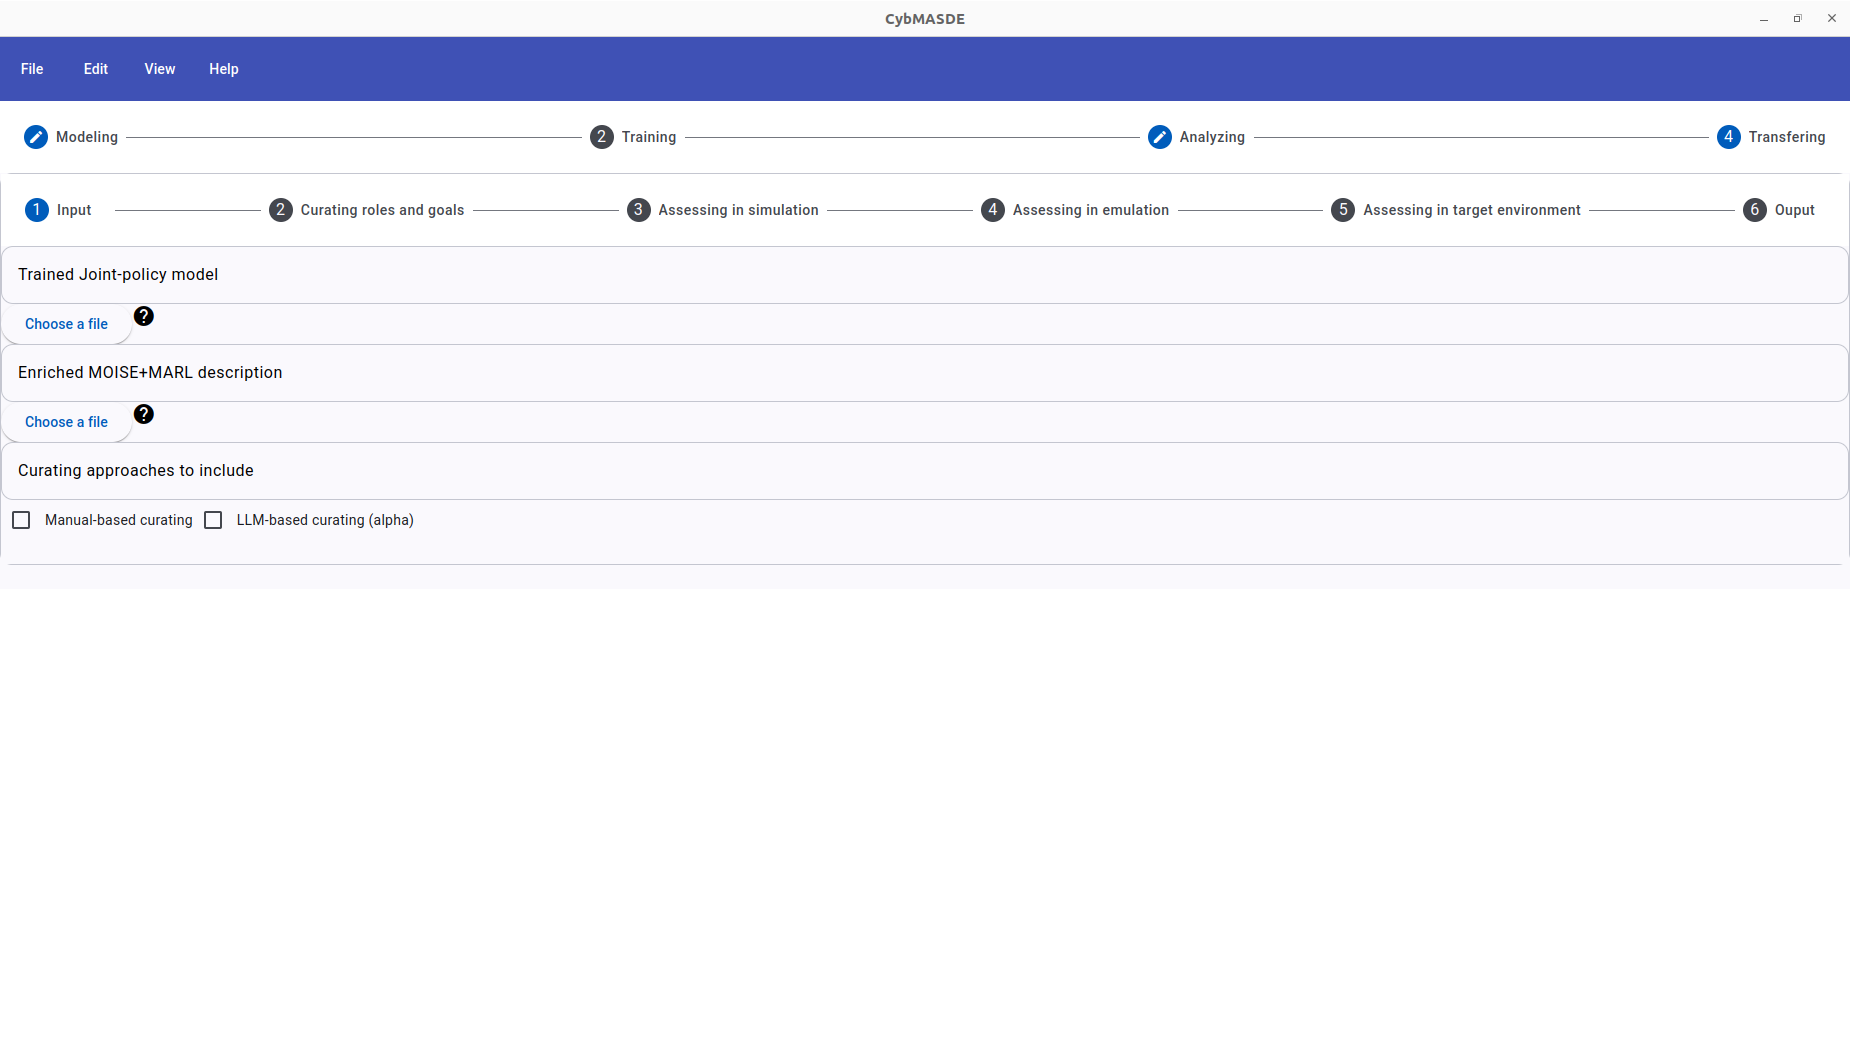
\includegraphics[trim=0cm 15cm 0cm 0cm, clip,width=\linewidth]{figures/refining.png}
       \caption[Screenshot of the refinement and transfer tab of the CybMASDE graphical interface]{Screenshot of the graphical interface for editing the CybMASDE project configuration file, showing the tab dedicated to the policy refinement and transfer phase. In this tab, the user can configure parameters related to multi-agent policy refinement, such as the maximum number of refinement iterations, termination criteria based on average reward and stability, and options for deploying policies in the real environment.}

       \label{fig:cybmasde_refining_screenshot}
\end{figure}
\clearpage
\section{CybMASDE Environmental API}\label{appendix:cybmasde-environment-api}
The \autoref{lst:cybmasde_environment_api} shows an excerpt from the template file to be used to implement the environmental API. This API is essential to enable \acn{CybMASDE} to communicate with the target environment. By implementing this interface, the user defines the methods necessary to retrieve observations and histories, apply joint actions, and deploy joint policies in the environment.
\begin{lstlisting}[language=Python,basicstyle=\scriptsize, label={lst:cybmasde_environment_api}, caption={Excerpt from the template file to be used to implement the environmental API.}]
class EnvironmentAPI:
“”“Class representing the environment API for interacting with the environment.”“”

def __init__(self):
pass
def retrieve_joint_observation(self):
“”“Retrieve the joint observation from the environment.”“”
# Implement the logic to retrieve the joint observation
pass
def retrieve_joint_histories(self):
‘’“Retrieve the joint histories from the environment.”“”
# Implement the logic to retrieve the joint histories

pass
def apply_joint_action(self, joint_action):
“”“Apply the joint action to the environment.”“”
# Implement the logic to apply the joint action
pass
def deploy_joint_policy(self, joint_policy):
‘’“Deploy the joint policy to the environment.”“”
# Implement the logic to deploy the joint policy
pass
\end {lstlisting}
\clearpage
\section{CybMASDE Command Line Manual}\label{appendix:cybmasde-manual}
\begin{verbatim}
CYBMASDE(1)                  Manuel de l'utilisateur                  CYBMASDE(1)
NOM
       cybmasde - orchestrer la méthode MAMAD pour la conception de SMA
SYNOPSIS
       cybmasde [commande] [options]
DESCRIPTION
       CybMASDE est une plateforme modulaire permettant de créer, configurer,
       valider, exécuter et analyser des projets de SMA fondés sur le cadre
       MOISE+MARL. Elle supporte l'exécution en ligne de commande (CLI) ou via
       son interface graphique Angular. Le CLI permet une automatisation
       complète (mode batch/HPC) ou une utilisation interactive.
COMMANDES PRINCIPALES
       init        Créer un nouveau projet et générer l'arborescence associée.
       validate    Vérifier la validité du fichier project_configuration.json et des dépendances.
       run         Exécuter un projet complet ou partiel.
       model       Lancer uniquement l'activité de modélisation.
       train       Lancer uniquement l'activité d'entraînement.
       analyze     Lancer uniquement l'activité d'analyse (Auto-TEMM).
       refine      Lancer un cycle de raffinement (analyse + entraînement).
       deploy      Déployer une politique dans l'environnement réel.
       status      Afficher l'état courant du projet (politiques, métriques, logs).
       clean       Nettoyer les fichiers temporaires, traces ou checkpoints inutiles.
       export      Exporter les résultats (politiques, métriques, specs. org.) au format JSON/CSV.
       help        Afficher l'aide générale ou celle d'une commande spécifique.
OPTIONS GÉNÉRALES
       -h, --help
              Afficher l'aide.
       -v, --version
              Afficher la version de CybMASDE.
       -p, --project <path>
              Chemin vers le projet (par défaut: répertoire courant).
       -c, --config <file>
              Spécifier un fichier de configuration alternatif.
SOUS-COMMANDES ET OPTIONS
   init
       cybmasde init -n <nom_projet> [-d <description>] [-o <output_dir>]
       -n, --name <nom>
              Nom du projet.
       -d, --description <texte>
              Description textuelle du projet.
       -o, --output <dir>
              Répertoire de sortie (par défaut: ./<nom_projet>).
       --template <type>
              Type de template d'environnement (handcrafted|worldmodel|minimal).
   validate
       cybmasde validate [-q]
       -q, --quiet
              Ne pas afficher les détails, seulement l'état final (OK/ERREUR).
       --strict
              Considérer tout avertissement comme une erreur.
   run
       cybmasde run [--full-auto | --semi-auto | --manual]
       --full-auto
              Exécuter l'ensemble du pipeline (MTA+T) sans interaction.
       --semi-auto
              Exécution complète mais pause à chaque étape pour confirmation.
       --manual
              Mode manuel : l'utilisateur choisit chaque activité à exécuter.
       --skip-model
              Ne pas relancer la modélisation (utiliser environnement existant).
       --skip-analyze
              Ne pas lancer Auto-TEMM même si la récompense est faible.
       --max-refine <N>
              Nombre maximal d'itérations de raffinement.
       --reward-threshold <val>
              Seuil de récompense moyenne pour arrêt automatique.
       --std-threshold <val>
              Seuil d'écart-type de la récompense pour arrêt du raffinement.
       --accept-inferred
              Accepter automatiquement les spécifications inférées sans validation humaine.
       --interactive-infer
              Afficher les specs inférées et demander validation manuelle (défaut).
   model
       cybmasde model [--auto | --manual] [options]
       --auto
              Utiliser les traces + World Model pour générer l'environnement.
       --manual
              Lancer l'environnement MCAS (handcrafted_environment.py).
       --traces <dir>
              Répertoire contenant des historiques préexistants.
       --vae-dim <val>
              Dimension latente des VAE (défaut: 32).
       --lstm-hidden <val>
              Taille des couches cachées LSTM (64 ou 128).
   train
       cybmasde train [--algo <alg>] [options]
       --algo <nom>
              Algorithme MARL (MAPPO|MADDPG|QMIX|IQL|VDN|ROMA).
       --batch-size <val>
              Taille des batchs (64 ou 128).
       --lr <val>
              Taux d'apprentissage (1e-4 à 5e-4).
       --gamma <val>
              Facteur de discount (0.9 à 0.99).
       --clip <val>
              Valeur de clipping PPO (0.1 à 0.3).
       --seed <val>
              Graine aléatoire.
       --epochs <N>
              Nombre d'époques.
   analyze
       cybmasde analyze [--auto-temm]
       --auto-temm
              Utiliser Auto-TEMM (clustering + optimisation hyperparamètres).
       --metrics <list>
              Sélectionner les métriques d'analyse (reward|stability|org_fit).
       --representativity <val>
              Seuil de représentativité (0.0–1.0).
   refine
       cybmasde refine [--max <N>] [--accept-inferred]
       --max <N>
              Nombre maximum d'itérations de raffinement.
       --accept-inferred
              Accepter automatiquement les specs organisationnelles inférées.
       --interactive
              Demander confirmation utilisateur à chaque cycle (défaut).
   deploy
       cybmasde deploy [--direct | --remote]
       --direct
              Déploiement de la politique sur les agents (mode embarqué).
       --remote
              Politique exécutée par CybMASDE, agents ne reçoivent que les actions.
       --checkpoint <file>
              Spécifier un checkpoint particulier de politique.
       --api <url>
              Spécifier l'URL de l'API environnementale cible.
   status
       cybmasde status
       Affiche l'état du projet : politique active, métriques récentes,
       nombre de cycles MTA, état du transfert.
   clean
       cybmasde clean [--traces | --checkpoints | --all]
       Nettoyer les fichiers temporaires et résultats intermédiaires.
   export
       cybmasde export [--format json|csv|yaml] [--output <dir>]
       Exporter les résultats, politiques et spécifications organisationnelles.
EXEMPLES
       cybmasde init -n infra_test --template worldmodel
       cybmasde validate
       cybmasde run --full-auto --reward-threshold 3.5 --max-refine 5
       cybmasde refine --interactive
       cybmasde deploy --remote --api http://localhost:8080/api
VOIR AUSSI
       Documentation complète : https://github.com/julien6/CybMASDE
       Référence théorique MAMAD et MOISE+MARL dans le manuscrit associé.
\end{verbatim}
